\documentclass[10pt]{beamer}
\usetheme{Singapore}
\usepackage[polish]{babel}
\usepackage[T1]{fontenc}
\usepackage[utf8x]{inputenc}
\usepackage{amsmath}
\usepackage{amsfonts}
\usepackage{amssymb}
\usepackage{graphicx}
\usepackage{caption}


\author{Klara Muzalewska}
\title{Modelowanie budynków\vspace{0.7cm}
 \\ "Chodź pomóż mi AI"}
%\setbeamercovered{transparent} 
%\setbeamertemplate{navigation symbols}{} 
%\logo{} 
%\subject{} 
\begin{document}

\begin{frame}

\titlepage
\end{frame}

\setbeamertemplate{section in toc}{\inserttocsectionnumber.~\inserttocsection}

\begin{frame}{Plan referatu}
 \tableofcontents[sections={1-4}]
\end{frame}

\section{Modelowanie budynku}

\begin{frame}{Modelowanie budynku}
\begin{tabular}{c c}

Building Information Modeling & Bridge Management Systems\\
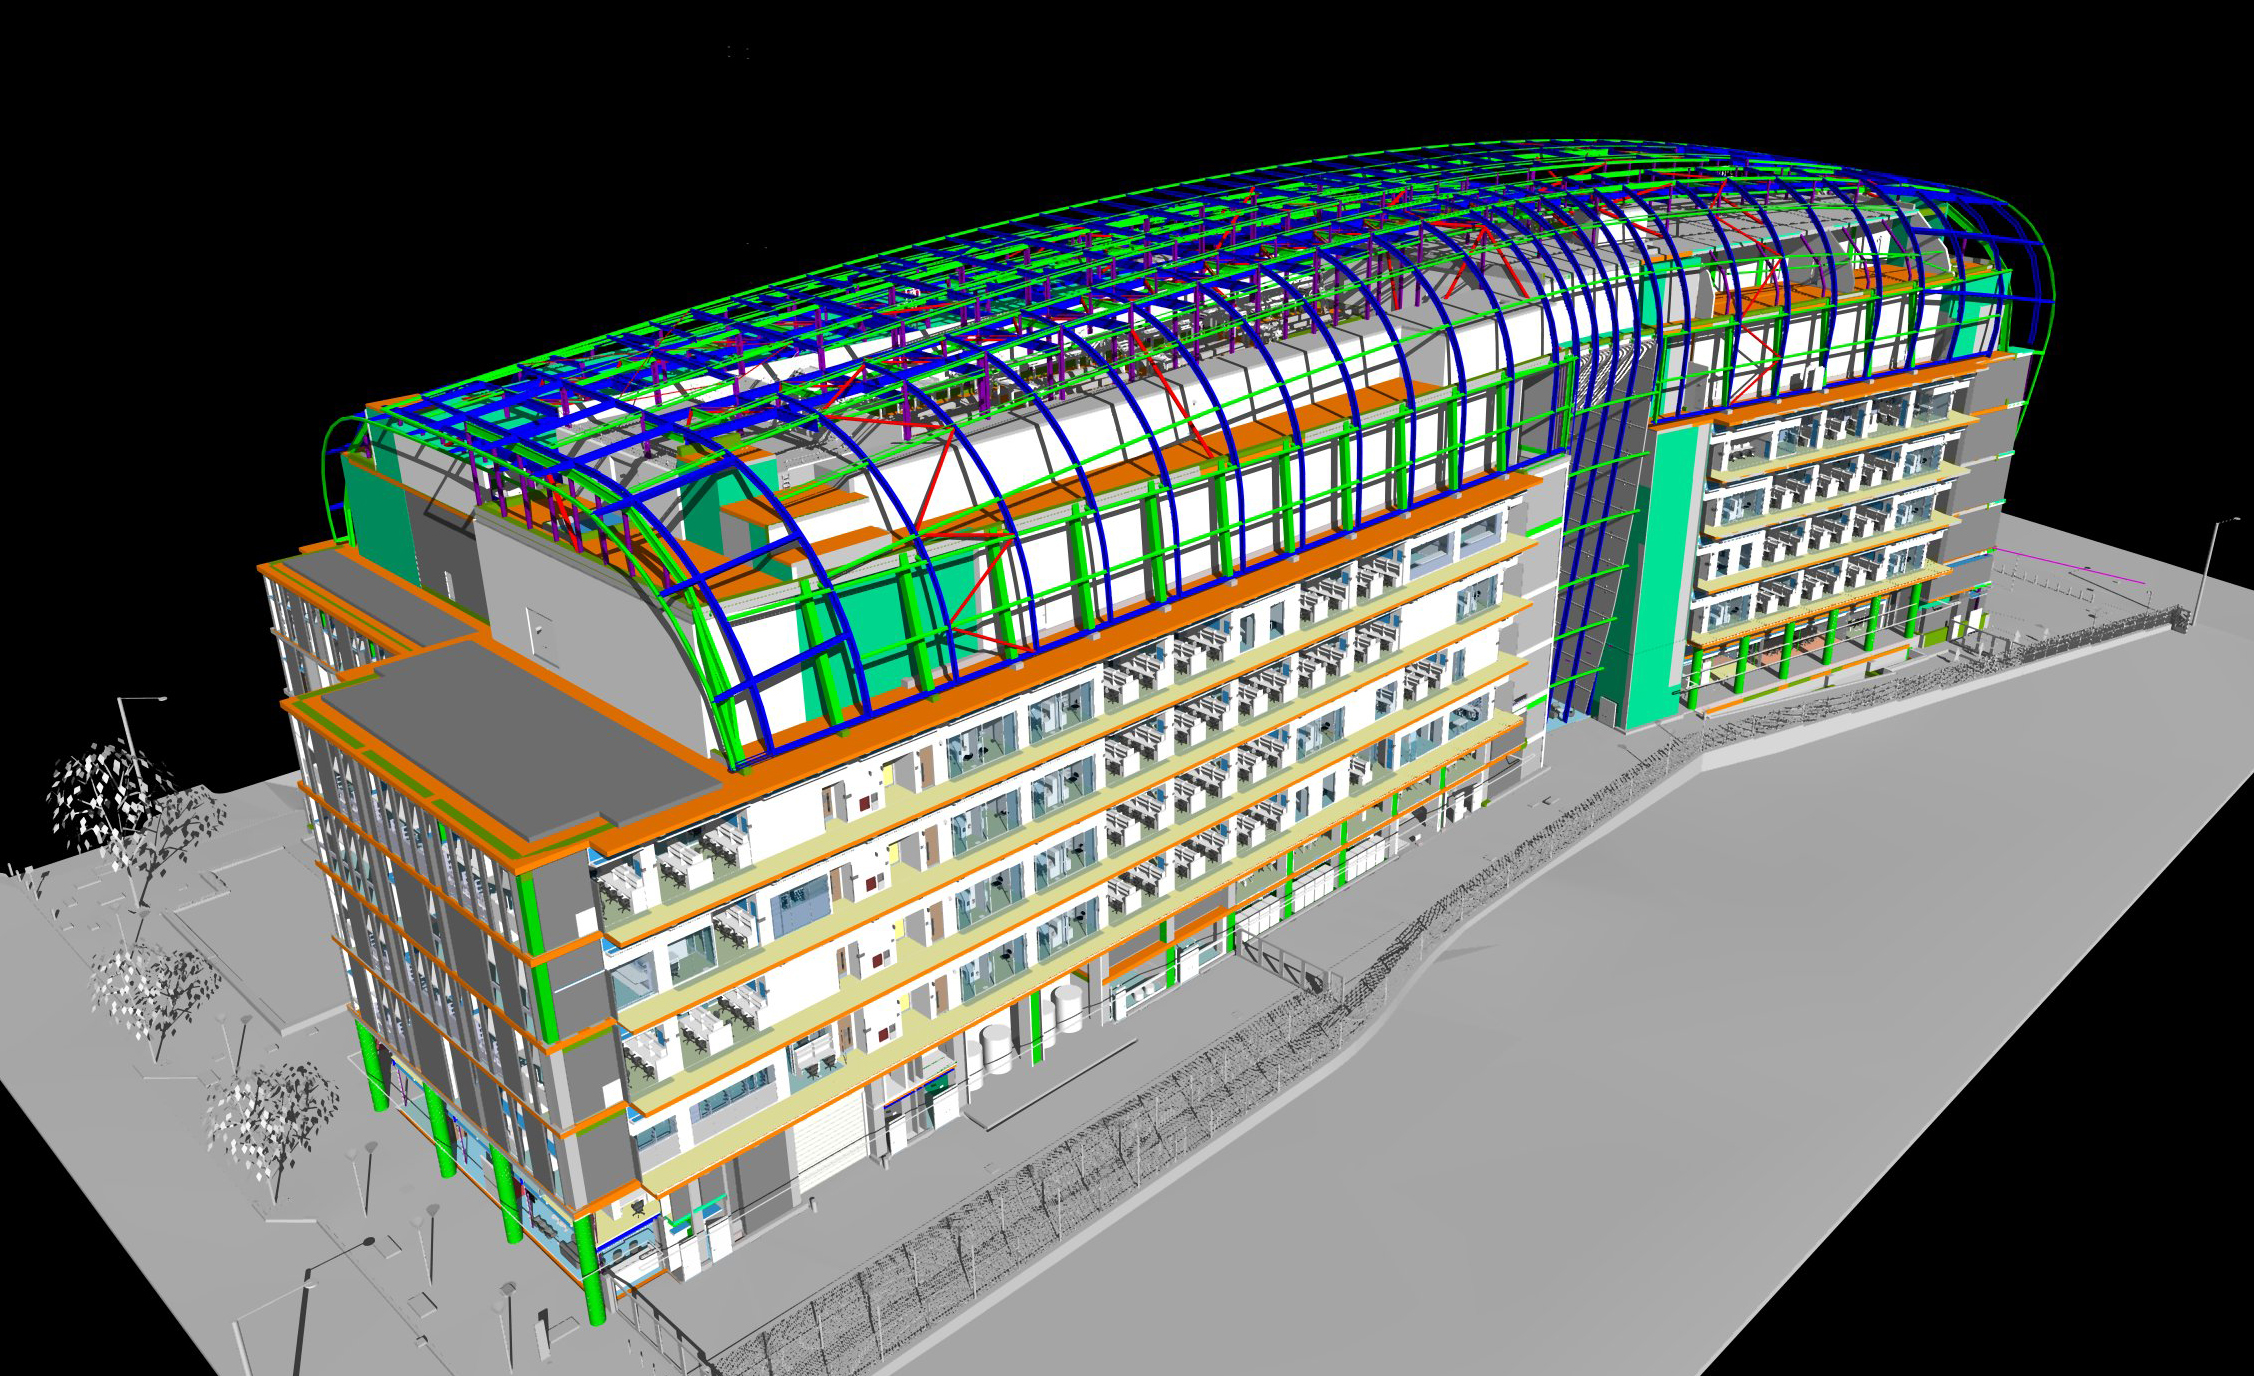
\includegraphics[scale=0.07]{bim.jpeg}

&


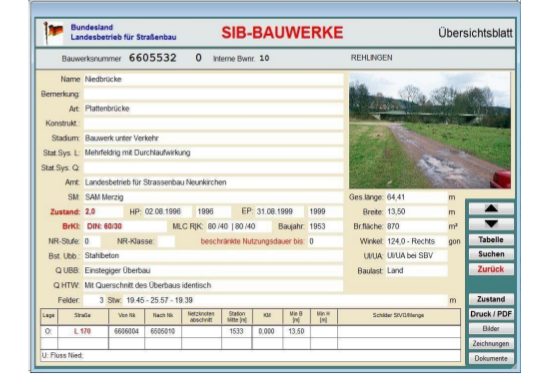
\includegraphics[scale=0.27]{BMS.png}


\end{tabular} 

\end{frame}

\section{Sztuczna inteligencja w modelowaniu}

\begin{frame}{Sztuczna inteligencja w modelowaniu}

\begin{block}{Sieć bayesowska}
\begin{itemize}
\item oparta na twierdzeniu Bayesa \\\begin{center}
$P(A|B)=\frac{P(B|A)P(A)}{P(B)}$
\end{center} 
\item sieć definiowana przez skierowany, acykliczny graf
\end{itemize}
\end{block}

\end{frame}

\begin{frame}{Sztuczna inteligencja w modelowaniu}
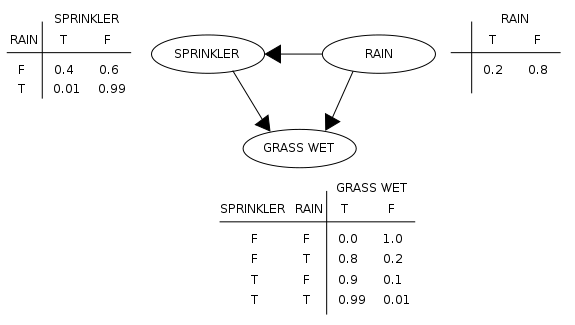
\includegraphics[scale=0.5]{bayes.png}
\end{frame}

\begin{frame}{Sztuczna inteligencja w modelowaniu}
\begin{itemize}
\item Pobieramy zestawy danych z BMS $\rightarrow$ struktura sieci, tabele
\item Wnioskowania probabilistyczne
\end{itemize}
\end{frame}



\begin{frame}{The Tree Augmented Naive Baye}
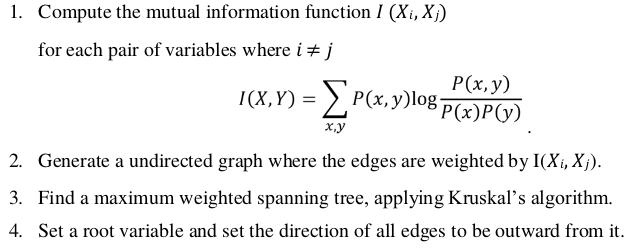
\includegraphics[scale=0.5]{TAN.png}
\end{frame}

\begin{frame}{Próbkowanie Gibbsa}
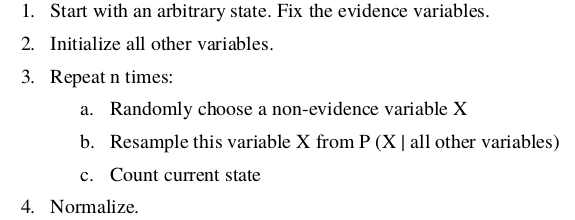
\includegraphics[scale=0.5]{Gibs.png}
\end{frame}

\section{Efekty}
\begin{frame}{Efekty}
\begin{itemize}
\item Wyniki były odpowiednie do zamodelowania pewnych mostów.
\item Aby uzyskać lepsze rady dotyczące projektowania należałoby dodać więcej danych i lepszą dyskretyzacja.
\item Aby uwzględnić kolejne procesy projektowania należałoby
uwzględnić kolejne czynniki, które możemy uzyskać również z BMS. 
\end{itemize}
\end{frame}



\section{Bibliografia}
\begin{frame}{Bibliografia}
"Knowledge based Bridge Engineering - Artificial Intelligence meets Building Information Modeling"\ Dominic Singer, Maximilian Bügler, André Borrmann	
\end{frame}


\begin{frame}{}
\begin{center}
\LARGE Dziękuje za uwage
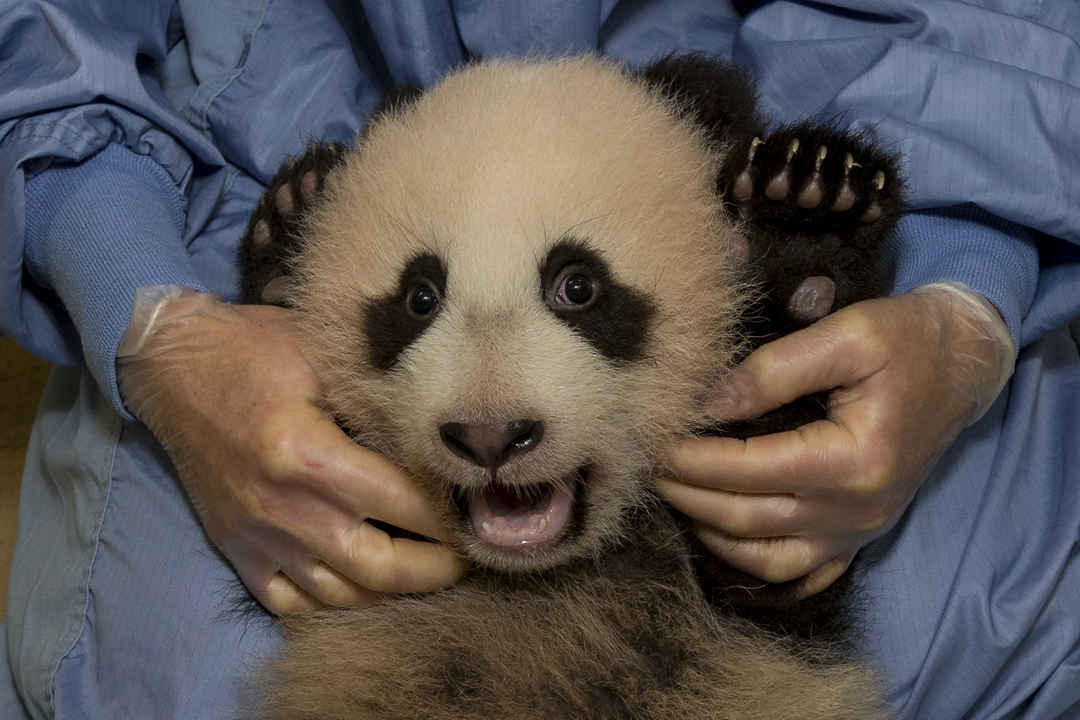
\includegraphics[scale=0.25]{Panda.jpg}
\end{center}
\end{frame}
\end{document}
